\documentclass[10pt]{beamer}
\usetheme[progressbar=frametitle]{metropolis}

\usepackage{appendixnumberbeamer}
\usepackage{booktabs}
\usepackage{pgfplots}
\usepgfplotslibrary{dateplot}
\usepackage{xspace}
\usepackage{amsmath}
\usepackage{amssymb}
\usepackage{subfig}
\usepackage{graphicx}
\usepackage{caption}
\usepackage{pdfpages}
\usepackage{multimedia}

\graphicspath{ {./images/} }

\newcommand{\themename}{\textbf{\textsc{metropolis}}\xspace}

\title{Brief discussion on evolution of GNSS}
\subtitle{Based on article "Evolution of the Global Navigation Satellite System (GNSS)"\\
Author: Christopher J. Hegarty  and Eric Chatre}
% \date{\today}
\date{}
\author{Aziel Martins de Freitas Júnior}
\institute{SENAI CIMATEC}
% \titlegraphic{\hfill\includegraphics[height=1.5cm]{logo.pdf}}

\begin{document}

\maketitle

%----------------------SLIDE 01----------------------%

\begin{frame}{Contents}

  \setbeamertemplate{section in toc}[sections numbered]
  \tableofcontents%[hideallsubsections]

\end{frame}

\section[Introduction]{Introduction}

%----------------------SLIDE 02----------------------%

\begin{frame}[fragile]{Motivation}
1
\end{frame}

%----------------------SLIDE 03----------------------%

\begin{frame}[fragile]{ARToolKit}
  \begin{columns}
    % Left column
    \column{0.5\textwidth}
    \begin{itemize}
      \item First article published in 1999;
      \item Intended for augmented reality in collaborative office work;
      \item One user would wear a HMD (\emph{head mounted display}) to provide others augmented reality visuals.
    \end{itemize}
    % Right column
    \column{0.5\textwidth}
      % \begin{figure}
      %   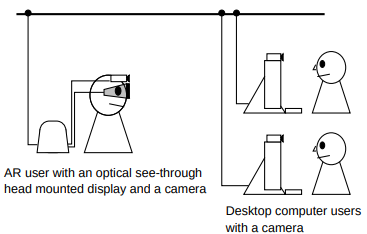
\includegraphics[scale=0.35]{1999-sysoverview}
      %   \caption{Intended usage.}
      % \end{figure}
      % \begin{figure}
      %   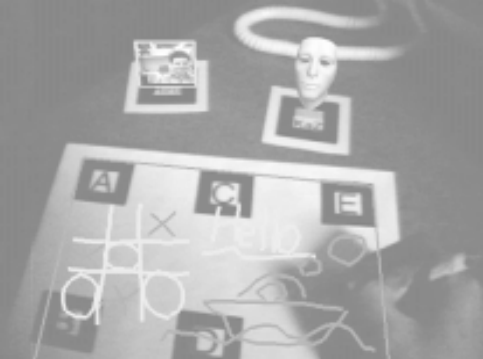
\includegraphics[scale=0.25]{1999-virtboard}
      %   \caption{HMD image.}
      % \end{figure}
  \end{columns}
\end{frame}

\end{document}